% move all configuration stuff into includes file so we can focus on the content
\documentclass[aspectratio=169,hyperref={pdfpagelabels=false,colorlinks=true,linkcolor=white,urlcolor=lightblue},xcolor={table},t]{beamer}

%%%%%%%%%%%%%%%%%%%%%%%%%%%%%%%%%%%%%%%%%%%%%%%%%%%%%%%%%%%%%%%%%%%%%%%%%%%%%%%%%%
%%%%%%%%%%%%%%%%%%%%%%%%%%%%%%%%%%%%%%%%%%%%%%%%%%%%%%%%%%%%%%%%%%%%%%%%%%%%%%%%%%
% packages
\usepackage{pict2e}
\usepackage{epic}
\usepackage{amsmath,amsfonts,amssymb}
\usepackage{units}
\usepackage{fancybox}
\usepackage[absolute,overlay]{textpos} 
%\usepackage[table]{xcolor}
\usepackage{animate}
\usepackage{gensymb}
%\usepackage{graphicx}
%\usepackage{longtable}
\usepackage{multirow}
\usepackage{silence}
\usepackage{tikz}
\usepackage[backend=bibtex,style=ieee]{biblatex}
\AtEveryCitekey{\iffootnote{\tiny}{}}
\addbibresource{include/references}



% fontsize
\let\Tiny=\tiny

%%%%%%%%%%%%%%%%%%%%%%%%%%%%%%%%%%%%%%%%%%%%%%%%%%%%%%%%%%%%%%%%%%%%%%%%%%%%%%%%%%
%%%%%%%%%%%%%%%%%%%%%%%%%%%%%%%%%%%%%%%%%%%%%%%%%%%%%%%%%%%%%%%%%%%%%%%%%%%%%%%%%%
% warnings
\pdfsuppresswarningpagegroup=1
\WarningFilter{biblatex}{Patching footnotes failed}
\WarningFilter{latexfont}{Font shape}
\WarningFilter{latexfont}{Some font shapes}
\WarningFilter{gensymb}{Not defining}


%%%%%%%%%%%%%%%%%%%%%%%%%%%%%%%%%%%%%%%%%%%%%%%%%%%%%%%%%%%%%%%%%%%%%%%%%%%%%%%%%%
%%%%%%%%%%%%%%%%%%%%%%%%%%%%%%%%%%%%%%%%%%%%%%%%%%%%%%%%%%%%%%%%%%%%%%%%%%%%%%%%%%
% theme & layout
\usetheme{Frankfurt}
\useinnertheme{rectangles}


%%%%%%%%%%%%%%%%%%%%%%%%%%%%%%%%%%%%%%%%%%%%%%%%%%%%%%%%%%%%%%%%%%%%%%%%%%%%%%%%%%
\setbeamertemplate{frametitle}[default][colsep=-4bp,rounded=false,shadow=false]
\setbeamertemplate{frametitle}
{%
    \nointerlineskip%
    %\vskip-0.5ex
    \begin{beamercolorbox}[wd=\paperwidth,ht=3.5ex,dp=0.6ex]{frametitle}
        \hspace*{1.3ex}\insertframetitle%
        
        \hspace*{1.3ex}\small\insertframesubtitle%
    \end{beamercolorbox}%
    \begin{textblock*}{100mm}(13.75cm,1cm)
        
\includegraphics[height=.4cm,keepaspectratio]{graph/Logo_GTCMT_white}
    \end{textblock*}
}


%%%%%%%%%%%%%%%%%%%%%%%%%%%%%%%%%%%%%%%%%%%%%%%%%%%%%%%%%%%%%%%%%%%%%%%%%%%%%%%%%%
\setbeamertemplate{title page}[default][colsep=-4bp,rounded=false,shadow=false]
\setbeamertemplate{title page}
{
    \begin{textblock*}{100mm}(15cm,.51cm)
            \href{https://github.com/alexanderlerch/ACA-Slides/blob/2nd_edition/\jobname.pdf}{\includegraphics[height=.5cm,keepaspectratio]{graph/Logo_github}}\hspace*{2ex}
    \end{textblock*}
    \begin{textblock*}{100mm}(15cm,1.3cm)
            \href{\IEEELink}{
\includegraphics[height=.5cm,keepaspectratio]{graph/icon/book}}\hspace*{2ex}
    \end{textblock*}
    \vskip-10ex
    \begin{beamercolorbox}[wd=\paperwidth,ht=.7\paperheight,dp=0.6ex]{frametitle} %35ex
        %\begin{flushright}
            %\href{http://www.gtcmt.gatech.edu}{
\includegraphics[height=.8cm,keepaspectratio]{graph/Logo_GTCMT_black}}\hspace*{2ex}
        %\end{flushright}
        
        \hspace*{1.8ex}\LARGE\inserttitle%
        
        \vspace*{.5ex}
        
        \hspace*{1.3ex}\small\insertsubtitle%
        
        \vspace*{.5ex}
    \end{beamercolorbox}%
    \nointerlineskip%
    \begin{beamercolorbox}[wd=\paperwidth,ht=.4\paperheight,dp=0.6ex]{page number in head/foot}
        %\vspace*{-.5ex}
        \hspace*{1.7ex}\small\insertauthor%
        
        %\hspace*{1.7ex}\small }%
        
        \vspace*{12ex}
        \vfill
        \begin{flushright}
            \href{http://www.gtcmt.gatech.edu}{
\includegraphics[height=.5cm,keepaspectratio]{graph/Logo_GTCMT_black}}\hspace*{2ex}
        \end{flushright}
    \end{beamercolorbox}%
}


%%%%%%%%%%%%%%%%%%%%%%%%%%%%%%%%%%%%%%%%%%%%%%%%%%%%%%%%%%%%%%%%%%%%%%%%%%%%%%%%%%
%\makeatother
\setbeamertemplate{footline}
{
  \leavevmode%
  \hbox{%
  \begin{beamercolorbox}[wd=.5\paperwidth,ht=2.25ex,dp=1ex,left,leftskip=1ex]{page number in head/foot}%
    \insertsubtitle
  \end{beamercolorbox}%
  \begin{beamercolorbox}[wd=.5\paperwidth,ht=2.25ex,dp=1ex,right,rightskip=1ex]{page number in head/foot}%
    \hfill
    \insertframenumber{} / \inserttotalframenumber
  \end{beamercolorbox}}%
  \vskip0pt%
}
%\makeatletter


%%%%%%%%%%%%%%%%%%%%%%%%%%%%%%%%%%%%%%%%%%%%%%%%%%%%%%%%%%%%%%%%%%%%%%%%%%%%%%%%%%
\beamertemplatenavigationsymbolsempty
\setbeamertemplate{navigation symbols}{}
\setbeamertemplate{blocks}[default]%[rounded=false,shadow=false]
\setbeamertemplate{itemize item}[square]
\setbeamertemplate{itemize subitem}[circle]
\setbeamertemplate{itemize subsubitem}[triangle]
\setbeamertemplate{enumerate item}[square]
\setbeamertemplate{enumerate subitem}[circle]
\setbeamertemplate{enumerate subsubitem}[circle]


%%%%%%%%%%%%%%%%%%%%%%%%%%%%%%%%%%%%%%%%%%%%%%%%%%%%%%%%%%%%%%%%%%%%%%%%%%%%%%%%%%
% colors
\setbeamercolor{structure}{fg=darkgray}
\setbeamercovered{transparent} %invisible
\setbeamercolor{bibliography entry author}{fg=black}
\setbeamercolor*{bibliography entry title}{fg=black}
\setbeamercolor*{bibliography entry note}{fg=black}
\setbeamercolor{frametitle}{fg=black}
\setbeamercolor{title}{fg=white}
\setbeamercolor{subtitle}{fg=white}
\setbeamercolor{frametitle}{fg=white}
\setbeamercolor{framesubtitle}{fg=white}
\setbeamercolor{mini frame}{fg=white, bg=black}
\setbeamercolor{section in head/foot}{fg=white, bg=darkgray}
\setbeamercolor{page number in head/foot}{fg=black, bg=lightblue}
\setbeamercolor{item projected}{fg=white, bg=black}

%---------------------------------------------------------------------------------
%%%%%%%%%%%%%%%%%%%%%%%%%%%%%%%%%%%%%%%%%%%%%%%%%%%%%%%%%%%%%%%%%%%%%%%%%%%%%%%%%%
%%%%%%%%%%%%%%%%%%%%%%%%%%%%%%%%%%%%%%%%%%%%%%%%%%%%%%%%%%%%%%%%%%%%%%%%%%%%%%%%%%
% title information
\title[]{Introduction to \textbf{Audio Content Analysis}}   
\author[alexander lerch]{alexander lerch} 
%\institute{~}
%\date[Alexander Lerch]{}
%\titlegraphic{\vspace{-16mm}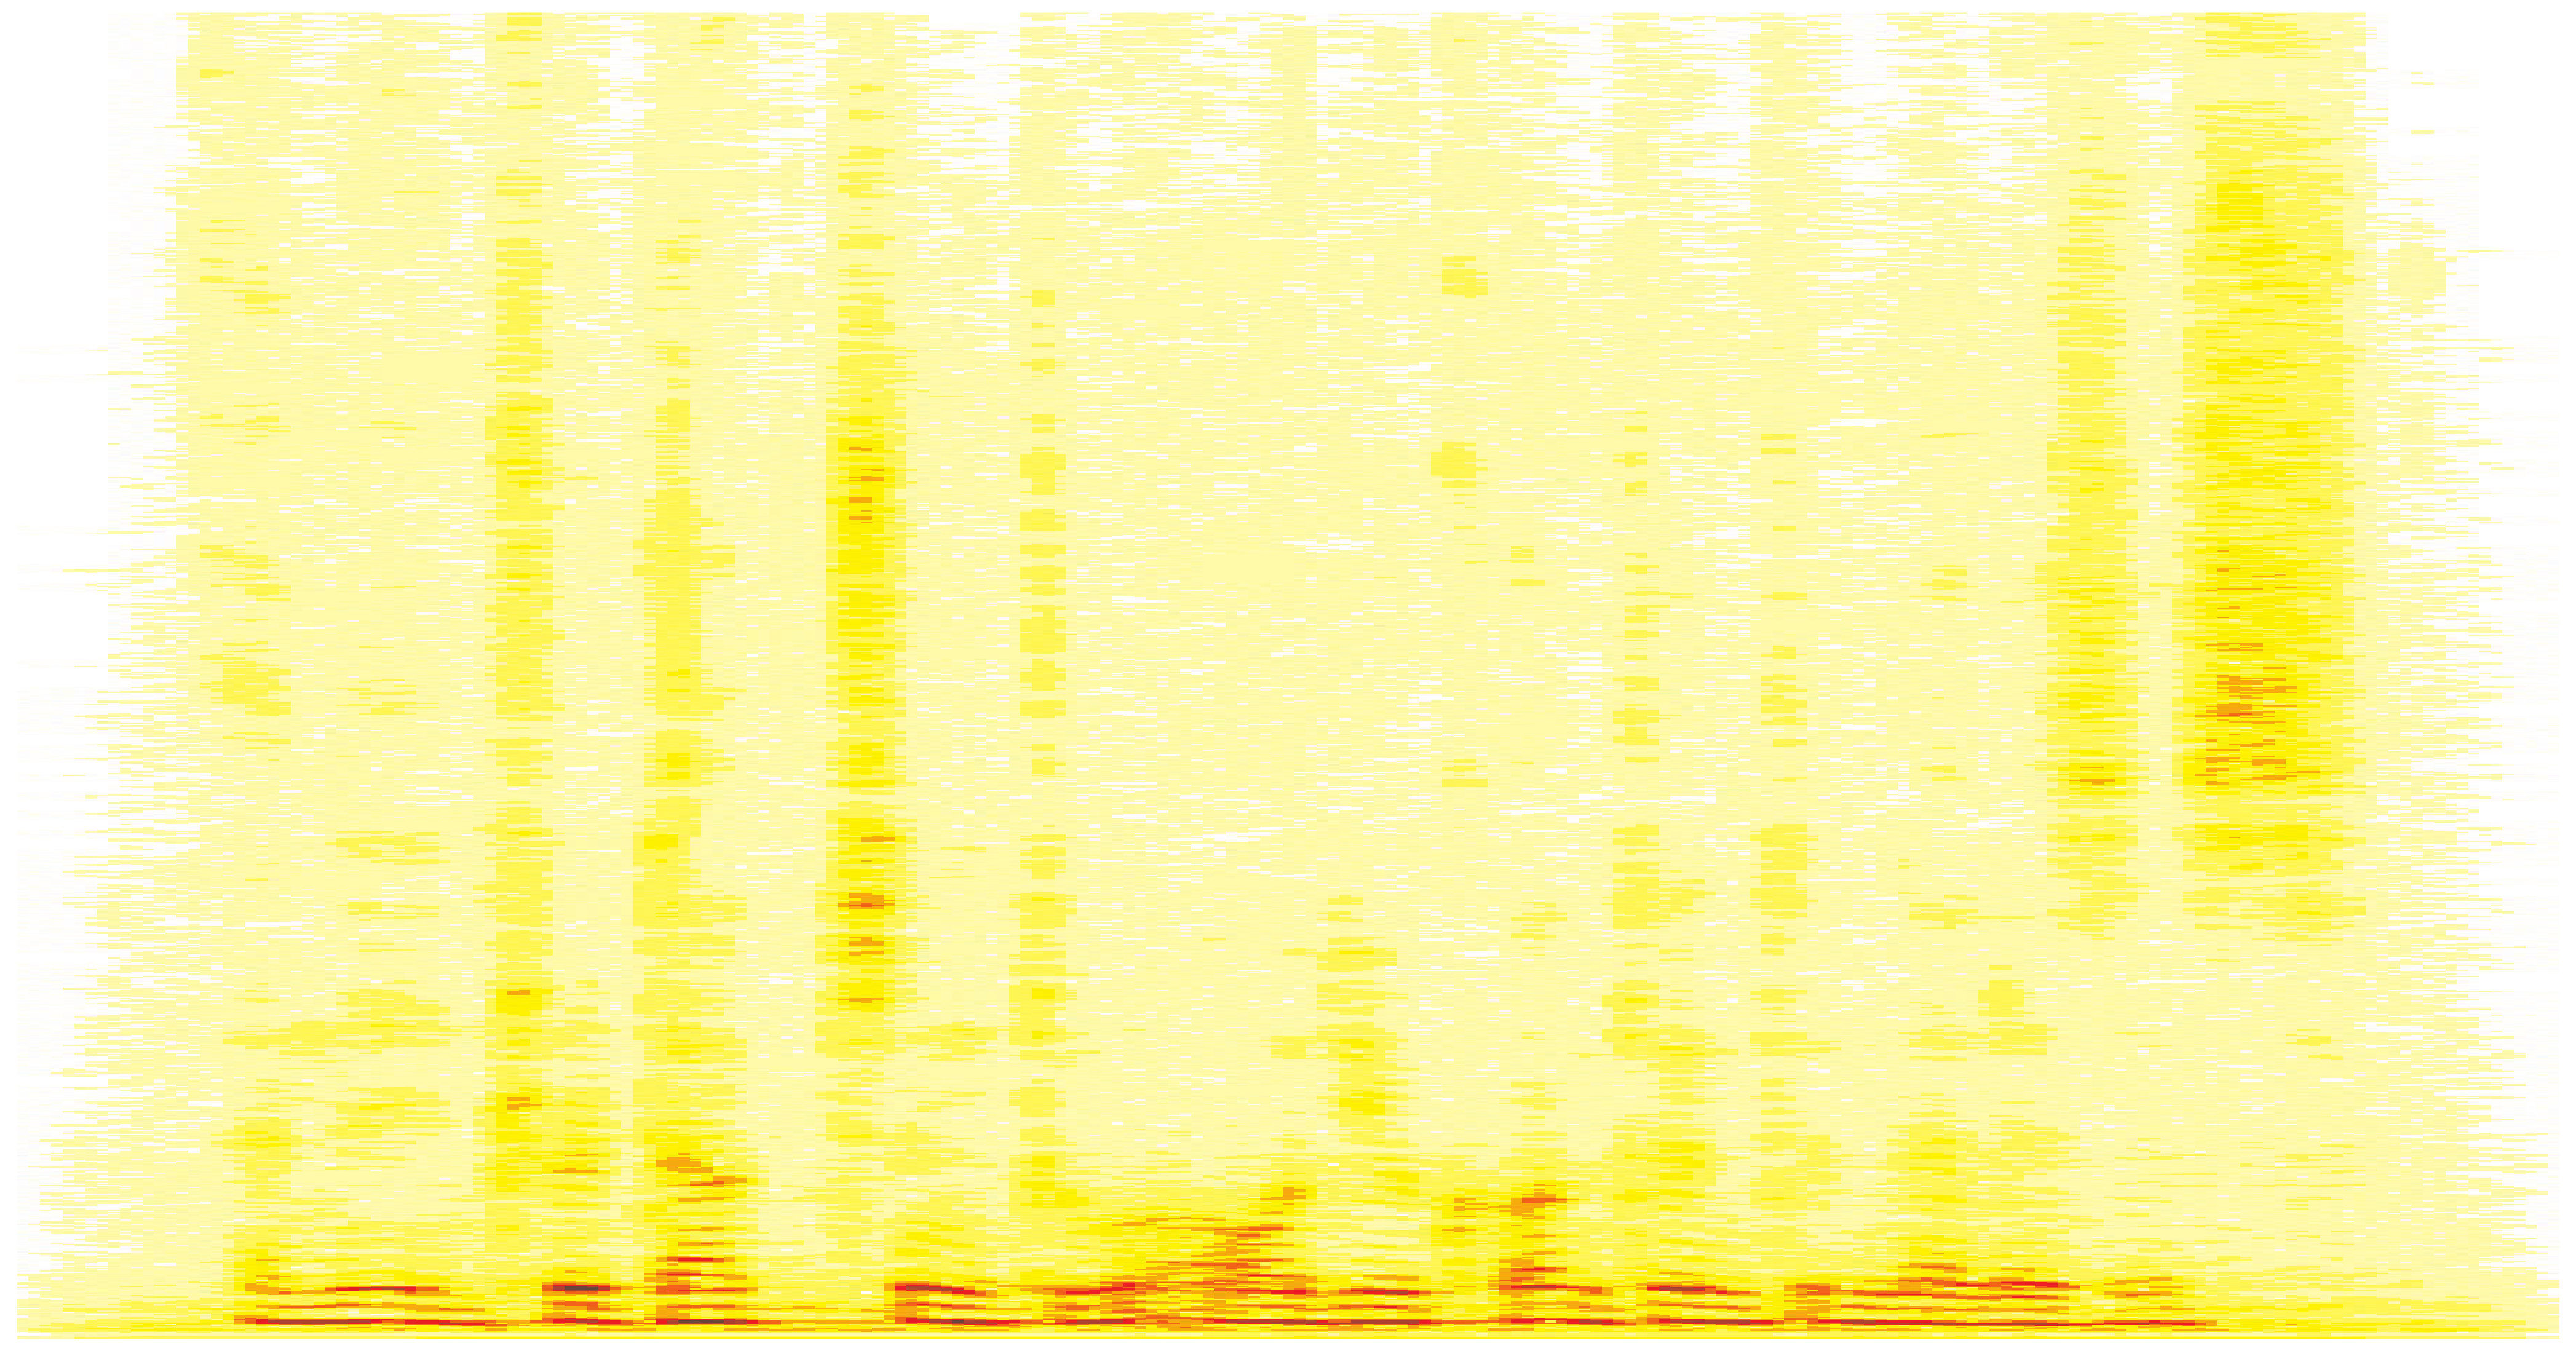
\includegraphics[width=\textwidth,height=3cm]{title}}

%%%%%%%%%%%%%%%%%%%%%%%%%%%%%%%%%%%%%%%%%%%%%%%%%%%%%%%%%%%%%%%%%%%%%%%%%%%%%%%%%%
%%%%%%%%%%%%%%%%%%%%%%%%%%%%%%%%%%%%%%%%%%%%%%%%%%%%%%%%%%%%%%%%%%%%%%%%%%%%%%%%%%
% colors
\definecolor{gtgold}{HTML}{96caff} %0e7eed {rgb}{0.88,0.66,1,0.06} [234, 170, 0]/256
\definecolor{darkgray}{rgb}{.1, .1, .25}
\definecolor{lightblue}{HTML}{0e7eed}
\definecolor{highlight}{rgb}{0, 0, 1} %_less!40

%%%%%%%%%%%%%%%%%%%%%%%%%%%%%%%%%%%%%%%%%%%%%%%%%%%%%%%%%%%%%%%%%%%%%%%%%%%%%%%%%%
%%%%%%%%%%%%%%%%%%%%%%%%%%%%%%%%%%%%%%%%%%%%%%%%%%%%%%%%%%%%%%%%%%%%%%%%%%%%%%%%%%
% relative paths
\graphicspath{{../ACA-Plots/graph/}}


%%%%%%%%%%%%%%%%%%%%%%%%%%%%%%%%%%%%%%%%%%%%%%%%%%%%%%%%%%%%%%%%%%%%%%%%%%%%%%%%%%
%%%%%%%%%%%%%%%%%%%%%%%%%%%%%%%%%%%%%%%%%%%%%%%%%%%%%%%%%%%%%%%%%%%%%%%%%%%%%%%%%%
% units
\setlength{\unitlength}{1mm}

%%%%%%%%%%%%%%%%%%%%%%%%%%%%%%%%%%%%%%%%%%%%%%%%%%%%%%%%%%%%%%%%%%%%%%%%%%%%%%%%%%
%%%%%%%%%%%%%%%%%%%%%%%%%%%%%%%%%%%%%%%%%%%%%%%%%%%%%%%%%%%%%%%%%%%%%%%%%%%%%%%%%%
% math
\DeclareMathOperator*{\argmax}{argmax}
\DeclareMathOperator*{\argmin}{argmin}
\DeclareMathOperator*{\atan}{atan}
\DeclareMathOperator*{\arcsinh}{arcsinh}
\DeclareMathOperator*{\sign}{sign}
\DeclareMathOperator*{\tcdf}{tcdf}
\DeclareMathOperator*{\si}{sinc}
\DeclareMathOperator*{\princarg}{princarg}
\DeclareMathOperator*{\arccosh}{arccosh}
\DeclareMathOperator*{\hwr}{HWR}
\DeclareMathOperator*{\flip}{flip}
\DeclareMathOperator*{\sinc}{sinc}
\DeclareMathOperator*{\floor}{floor}
\newcommand{\e}{{e}}
\newcommand{\jom}{\mathrm{j}\omega}
\newcommand{\jOm}{\mathrm{j}\Omega}
\newcommand   {\mat}[1]    		{\boldsymbol{\uppercase{#1}}}		%bold
\renewcommand {\vec}[1]    		{\boldsymbol{\lowercase{#1}}}		%bold

%%%%%%%%%%%%%%%%%%%%%%%%%%%%%%%%%%%%%%%%%%%%%%%%%%%%%%%%%%%%%%%%%%%%%%%%%%%%%%%%%%
%%%%%%%%%%%%%%%%%%%%%%%%%%%%%%%%%%%%%%%%%%%%%%%%%%%%%%%%%%%%%%%%%%%%%%%%%%%%%%%%%%
% media9
\newcommand{\includeaudio}[1]{
\href{run:audio/#1.mp3}{
\includegraphics[width=5mm, height=5mm]{graph/SpeakerIcon}}}

\newcommand{\includeanimation}[4]{{\begin{center}
                        \animategraphics[autoplay,loop,scale=.7]{#4}{animation/#1-}{#2}{#3}        
                        \end{center}
                        \addreference{matlab source: \href{https://github.com/alexanderlerch/ACA-Plots/blob/master/matlab/animate#1.m}{matlab/animate#1.m}}}
                        \inserticon{video}}
                        
%%%%%%%%%%%%%%%%%%%%%%%%%%%%%%%%%%%%%%%%%%%%%%%%%%%%%%%%%%%%%%%%%%%%%%%%%%%%%%%%%%
%%%%%%%%%%%%%%%%%%%%%%%%%%%%%%%%%%%%%%%%%%%%%%%%%%%%%%%%%%%%%%%%%%%%%%%%%%%%%%%%%%
% other commands
\newcommand{\question}[1]{%\vspace{-4mm}
                          \setbeamercovered{invisible}
                          \begin{columns}[T]
                            \column{.9\textwidth}
                                \textbf{#1}
                            \column{.1\textwidth}
                                \vspace{-8mm}
                                \begin{flushright}
                                     
\includegraphics[width=.9\columnwidth]{graph/question_mark}
                                \end{flushright}
                                \vspace{6mm}
                          \end{columns}\pause\vspace{-12mm}}

\newcommand{\toremember}[1]{
                        \inserticon{lightbulb}
                        }

\newcommand{\matlabexercise}[1]{%\vspace{-4mm}
                          \setbeamercovered{invisible}
                          \begin{columns}[T]
                            \column{.8\textwidth}
                                \textbf{matlab exercise}: #1
                            \column{.2\textwidth}
                                \begin{flushright}
                                     
\includegraphics[scale=.5]{graph/logo_matlab}
                                \end{flushright}
                                %\vspace{6mm}
                          \end{columns}}

\newcommand{\addreference}[1]{  
                  
                    \begin{textblock*}{\baselineskip }(.98\paperwidth,.5\textheight) %(1.15\textwidth,.4\textheight)
                         \begin{minipage}[b][.5\paperheight][b]{1cm}%
                            \vfill%
                             \rotatebox{90}{\tiny {#1}}
                        \end{minipage}
                   \end{textblock*}
                    }
                    
\newcommand{\figwithmatlab}[1]{
                    \begin{figure}
                        \centering
                        \includegraphics[scale=.7]{#1}
                        %\label{fig:#1}
                    \end{figure}
                    
                    \addreference{matlab source: \href{https://github.com/alexanderlerch/ACA-Plots/blob/main/matlab/plot#1.m}{plot#1.m}}}
\newcommand{\figwithref}[2]{
                    \begin{figure}
                        \centering
                        \includegraphics[scale=.7]{#1}
                        \label{fig:#1}
                    \end{figure}
                    
                    \addreference{#2}}  
                                    
\newcommand{\inserticon}[1]{
                    \begin{textblock*}{100mm}(14.5cm,7.5cm)
                        \includegraphics[height=.8cm,keepaspectratio]{graph/#1}
                    \end{textblock*}}            

%%%%%%%%%%%%%%%%%%%%%%%%%%%%%%%%%%%%%%%%%%%%%%%%%%%%%%%%%%%%%%%%%%%%%%%%%%%%%%%%%%
%%%%%%%%%%%%%%%%%%%%%%%%%%%%%%%%%%%%%%%%%%%%%%%%%%%%%%%%%%%%%%%%%%%%%%%%%%%%%%%%%%
% counters
\newcounter{i}
\newcounter{j}
\newcounter{iXOffset}
\newcounter{iYOffset}
\newcounter{iXBlockSize}
\newcounter{iYBlockSize}
\newcounter{iYBlockSizeDiv2}
\newcounter{iXBlockSizeDiv2}
\newcounter{iDistance}

\newcommand{\IEEELink}{https://ieeexplore.ieee.org/servlet/opac?bknumber=9965970}




\subtitle{module 12.2: musical genre classification}

%%%%%%%%%%%%%%%%%%%%%%%%%%%%%%%%%%%%%%%%%%%%%%%%%%%%%%%%%%%%%%%%%%%%%%%%%%%%
\begin{document}
    % generate title page
	{
\setbeamertemplate{headline}{} 
\setbeamertemplate{footline}{} 
\begin{frame}
    \titlepage
    %\vspace{-5mm}
\end{frame}
}
\addtocounter{framenumber}{-1}


    \section[overview]{lecture overview}
        \begin{frame}{introduction}{overview}
            \begin{block}{corresponding textbook section}
                    %\href{http://ieeexplore.ieee.org/xpl/articleDetails.jsp?arnumber=6331125}{Chapter 8: Musical Genre, Similarity, and Mood} (pp.~151--155)
                    section~12.2
            \end{block}

            \begin{itemize}
                \item   \textbf{lecture content}
                    \begin{itemize}
                        \item   musical genre
                        \item   processing steps in basic genre classifiers
                        \item   example: genre classification with a kNN
                    \end{itemize}
                \bigskip
                \item<2->   \textbf{learning objectives}
                    \begin{itemize}
                        \item   discuss ambiguities in the definition of musical genre and the possible impact on automatic systems
                        \item   describe the processing steps for traditional musical genre classifiers
                        \item   implement your own music genre classifier with Matlab
                    \end{itemize}
            \end{itemize}
            \inserticon{directions}
        \end{frame}

    \section[intro]{introduction}
        \begin{frame}{musical genre classification}{introduction}
            \begin{itemize}
                \item	one of the early/\textbf{seminal research topics} in MIR
                \bigskip
                \item<2->	classic \textit{machine learning }task
                    \begin{itemize}
                        \item   features $\rightarrow$ classification
                    \end{itemize}
                \bigskip
                \item<3->	\textbf{related tasks}:
                    \begin{itemize}
                        \item	speech-music classification
                        \item	instrument recognition
                        \item   artist identification
                        \item   music emotion recognition
                    \end{itemize}
            \end{itemize}
        \end{frame}

        \begin{frame}{musical genre classification}{applications}
            \begin{itemize}
                \item	large music databases:
                    \begin{itemize}
                        \item	annotation
                        \item	sorting, browsing, retrieving
                    \end{itemize}
                \bigskip
                \pause
                \item   recommendation and music discovery systems
                \item	automatic playlist generation
                \item	improving downstream MIR tasks by using side information/conditioning
            \end{itemize}
        \end{frame}

    \section[genre]{musical genre}
        \begin{frame}{musical genre classification}{genre: definition}
            \question{what is \textit{musical genre}}

            \bigskip
            \begin{itemize}
                \item   clusters of musical similarity?
                \item[$\rightarrow$]<2->             hard to answer in general, there are many \textbf{systematic problems}
                \smallskip
                    \begin{enumerate}
                        \item<3->	\textbf{non-agreement on taxonomies}
                            \begin{itemize}
                                \item   e.g., AllMusic vs.\ Pandora
                            \end{itemize}
                        \item<3->   \textbf{genre label scope}
                            \begin{itemize}
                                \item   e.g., song, album, artist, piece of a song
                            \end{itemize}
                        \item<3->	\textbf{ill-defined genre labels}
                            \begin{itemize}
                                \item   e.g., geographic (\textit{indian music}), historic (\textit{baroque}), technical (\textit{barbershop}), instrumentation (\textit{symphonic music}), usage (\textit{christmas songs})
                            \end{itemize}
                        \item<3->	\textbf{taxonomy scalability}
                            \begin{itemize}
                                \item   e.g., genres and subgenres evolve over time
                            \end{itemize}
                        \item<3->	\textbf{non-orthogonality} 
                            \begin{itemize}
                                \item   e.g., several genres for one piece of music
                            \end{itemize}
                    \end{enumerate}

            \end{itemize}
            
        \end{frame}
        \begin{frame}{musical genre classification}{genre: taxonomy examples}
                \vspace{-20mm}
                \begin{center}
                \scalebox{.7}
                {
                    				\begin{footnotesize}
					\begin{picture}(150,120)
						%%%%%%%%%%%%%%%%%%%%%%%%%%%%%%%%%%%%%%%%%%%
						%tzanetakis
						\setcounter{iXOffset}{0}
						\put(\value{iXOffset}, 83) {\text{{\shortstack[c]{Speech}}}}
						\put(\value{iXOffset}, 41) {\text{{\shortstack[c]{Music}}}}

						\addtocounter{iXOffset}{10} %10
						\put(\value{iXOffset},49) {\line(1,7){4}}
						\put(\value{iXOffset},48) {\line(1,6){4}}
						\put(\value{iXOffset},47) {\line(1,5){3.5}}
						\put(\value{iXOffset},46) {\line(1,4){3.5}}
						\put(\value{iXOffset},45) {\line(1,3){3.5}}
						\put(\value{iXOffset},44) {\line(1,2){3.5}}
						\put(\value{iXOffset},43) {\line(1,1){3.5}}
						\put(\value{iXOffset},42) {\line(1,-1){3.5}}
						\put(\value{iXOffset},41) {\line(1,-5){3.5}}

						\addtocounter{iXOffset}{1} %11
						\put(\value{iXOffset},85) {\line(1,1){3.5}}
						\put(\value{iXOffset},84) {\line(1,0){3}}
						\put(\value{iXOffset},83) {\line(1,-1){3.5}}
						
						%%%%%%%%%%%%%%%%%%%%%%%%%%%%%%%%%%%%%%%%%%%
						\setcounter{iXOffset}{15}
						\put(\value{iXOffset}, 87) {\text{{\shortstack[c]{Male}}}}
						\put(\value{iXOffset}, 83) {\text{{\shortstack[c]{Female}}}}
						\put(\value{iXOffset}, 79) {\text{{\shortstack[c]{Sports}}}}
						\put(\value{iXOffset}, 75) {\text{{\shortstack[c]{Disco}}}}
						\put(\value{iXOffset}, 71) {\text{{\shortstack[c]{Country}}}}
						\put(\value{iXOffset}, 67) {\text{{\shortstack[c]{Hip Hop}}}}
						\put(\value{iXOffset}, 63) {\text{{\shortstack[c]{Rock}}}}
						\put(\value{iXOffset}, 59) {\text{{\shortstack[c]{Blues}}}}
						\put(\value{iXOffset}, 55) {\text{{\shortstack[c]{Reggae}}}}
						\put(\value{iXOffset}, 51) {\text{{\shortstack[c]{Pop}}}}
						\put(\value{iXOffset}, 47) {\text{{\shortstack[c]{Metal}}}}
						\put(\value{iXOffset}, 37) {\text{{\shortstack[c]{Classical}}}}
						\put(\value{iXOffset}, 17) {\text{{\shortstack[c]{Jazz}}}}
					
						\addtocounter{iXOffset}{8} %28
						\put(\value{iXOffset},20) {\line(1,0.8){8}}
						\put(\value{iXOffset},19) {\line(1,0.5){8}}
						\put(\value{iXOffset},18) {\line(1,0.1){8}}
						\put(\value{iXOffset},17) {\line(1,-0.2){8}}
						\put(\value{iXOffset},16) {\line(1,-0.5){8}}
						\put(\value{iXOffset},15) {\line(1,-0.8){8}}
					
						\addtocounter{iXOffset}{5} %28
						\put(\value{iXOffset},39) {\line(1,1){3.5}}
						\put(\value{iXOffset},38) {\line(1,0.5){3}}
						\put(\value{iXOffset},37) {\line(1,-0.3){3.5}}
						\put(\value{iXOffset},36) {\line(1,-1){3.5}}
					
						%%%%%%%%%%%%%%%%%%%%%%%%%%%%%%%%%%%%%%%%%%%
						\setcounter{iXOffset}{33}
						\put(\value{iXOffset}, 43) {\text{{\shortstack[c]{Choir}}}}
						\put(\value{iXOffset}, 39) {\text{{\shortstack[c]{Orchestra}}}}
						\put(\value{iXOffset}, 35) {\text{{\shortstack[c]{Piano}}}}
						\put(\value{iXOffset}, 31) {\text{{\shortstack[c]{String Quartet}}}}
						\put(\value{iXOffset}, 27) {\text{{\shortstack[c]{Big Band}}}}
						\put(\value{iXOffset}, 23) {\text{{\shortstack[c]{Cool}}}}
						\put(\value{iXOffset}, 19) {\text{{\shortstack[c]{Fusion}}}}
						\put(\value{iXOffset}, 15) {\text{{\shortstack[c]{Piano}}}}
						\put(\value{iXOffset}, 11) {\text{{\shortstack[c]{Quartet}}}}
						\put(\value{iXOffset}, 7) {\text{{\shortstack[c]{Swing}}}}

						%%%%%%%%%%%%%%%%%%%%%%%%%%%%%%%%%%%%%%%%%%%
						%burred
						\setcounter{iXOffset}{80}
						\put(\value{iXOffset}, 71) {\text{{\shortstack[c]{Background}}}}
						\put(\value{iXOffset}, 63) {\text{{\shortstack[c]{Speech}}}}
						\put(\value{iXOffset}, 27) {\text{{\shortstack[c]{Music}}}}

						\addtocounter{iXOffset}{11} 
						
						\put(\value{iXOffset},65) {\line(1,0.4){8}}
						\put(\value{iXOffset},64) {\line(1,0){8}}
						\put(\value{iXOffset},63) {\line(1,-0.4){8}}

						\addtocounter{iXOffset}{-1} 
						
						\put(\value{iXOffset},29) {\line(1,1.3){8}}
						\put(\value{iXOffset},27) {\line(1,-1){8}}
						
						%%%%%%%%%%%%%%%%%%%%%%%%%%%%%%%%%%%%%%%%%%%
						\addtocounter{iXOffset}{10} %100
						\put(\value{iXOffset}, 67) {\text{{\shortstack[c]{Male}}}}
						\put(\value{iXOffset}, 63) {\text{{\shortstack[c]{Female}}}}
						\put(\value{iXOffset}, 59) {\text{{\shortstack[c]{+Background}}}}
						\put(\value{iXOffset}, 42) {\text{{\shortstack[c]{Classical}}}}
						\put(\value{iXOffset}, 16) {\text{{\shortstack[c]{Non-Classical}}}}
						
						\addtocounter{iXOffset}{15} 
						\put(\value{iXOffset},44) {\line(1,1){6}}
						\put(\value{iXOffset},42) {\line(1,-0.8){6}}

						\addtocounter{iXOffset}{5} 
						\put(\value{iXOffset},18) {\line(1,3){2}}
						\put(\value{iXOffset},17) {\line(1,-0.1){2}}
						\put(\value{iXOffset},16) {\line(1,-3){2}}
						
						
						%%%%%%%%%%%%%%%%%%%%%%%%%%%%%%%%%%%%%%%%%%%
						\addtocounter{iXOffset}{3} % 123
						\put(\value{iXOffset}, 49) {\text{{\shortstack[c]{Chamber}}}}
						\put(\value{iXOffset}, 35) {\text{{\shortstack[c]{Orchestra}}}}
						\put(\value{iXOffset}, 25) {\text{{\shortstack[c]{Rock}}}}
						\put(\value{iXOffset}, 15) {\text{{\shortstack[c]{Electro/Pop}}}}
						\put(\value{iXOffset}, 7) {\text{{\shortstack[c]{Jazz/Blues}}}}

						\addtocounter{iXOffset}{8} %131
						\put(\value{iXOffset},27) {\line(1,0.1){10}}
						\put(\value{iXOffset},25) {\line(1,-0.1){10}}

						\addtocounter{iXOffset}{6} %137
						\put(\value{iXOffset},52) {\line(1,0.8){4}}
						\put(\value{iXOffset},51) {\line(1,0.1){4}}
						\put(\value{iXOffset},50) {\line(1,-0.2){4}}
						\put(\value{iXOffset},49) {\line(1,-1){4}}
											
						\addtocounter{iXOffset}{1} %138
						\put(\value{iXOffset},37) {\line(1,0.7){4}}
						\put(\value{iXOffset},36) {\line(1,0){4}}
						\put(\value{iXOffset},35) {\line(1,-0.7){4}}
											
						\addtocounter{iXOffset}{3} %141
						\put(\value{iXOffset},17) {\line(1,1){2}}
						\put(\value{iXOffset},16) {\line(1,0){2}}
						\put(\value{iXOffset},15) {\line(1,-1){2}}
						
						%%%%%%%%%%%%%%%%%%%%%%%%%%%%%%%%%%%%%%%%%%%
						\addtocounter{iXOffset}{3}
						\put(\value{iXOffset}, 55) {\text{{\shortstack[c]{Piano}}}}
						\put(\value{iXOffset}, 51) {\text{{\shortstack[c]{Solo}}}}
						\put(\value{iXOffset}, 47) {\text{{\shortstack[c]{String Quartet}}}}
						\put(\value{iXOffset}, 43) {\text{{\shortstack[c]{Other}}}}
						\put(\value{iXOffset}, 39) {\text{{\shortstack[c]{Symphonic}}}}
						\put(\value{iXOffset}, 35) {\text{{\shortstack[c]{+Choir}}}}
						\put(\value{iXOffset}, 31) {\text{{\shortstack[c]{+Soloist}}}}
						\put(\value{iXOffset}, 27) {\text{{\shortstack[c]{Soft Rock}}}}
						\put(\value{iXOffset}, 23) {\text{{\shortstack[c]{Hard Rock}}}}
						\put(\value{iXOffset}, 19) {\text{{\shortstack[c]{Hip Hop}}}}
						\put(\value{iXOffset}, 15) {\text{{\shortstack[c]{Techno/Dance}}}}
						\put(\value{iXOffset}, 11) {\text{{\shortstack[c]{Pop}}}}
					\end{picture}
				\end{footnotesize}

                }
                \end{center}
        \end{frame}

        \begin{frame}{musical genre classification}{observations with humans}
            \vspace{-3mm}
            \begin{columns}
                \column{.5\linewidth}
                    \begin{enumerate}
                        \item   human classification far from perfect: \unit[75--90]{\%} for limited set of classes
                        \item<2-> for many genres, humans need only a fraction of a second to classify
                        \smallskip
                        \item<2->[$\Rightarrow$]	short time timbre features sufficient?
                    \end{enumerate}
                \column{.5\linewidth}
                    \begin{figure}
                        \centering
                        \only<1>{
                            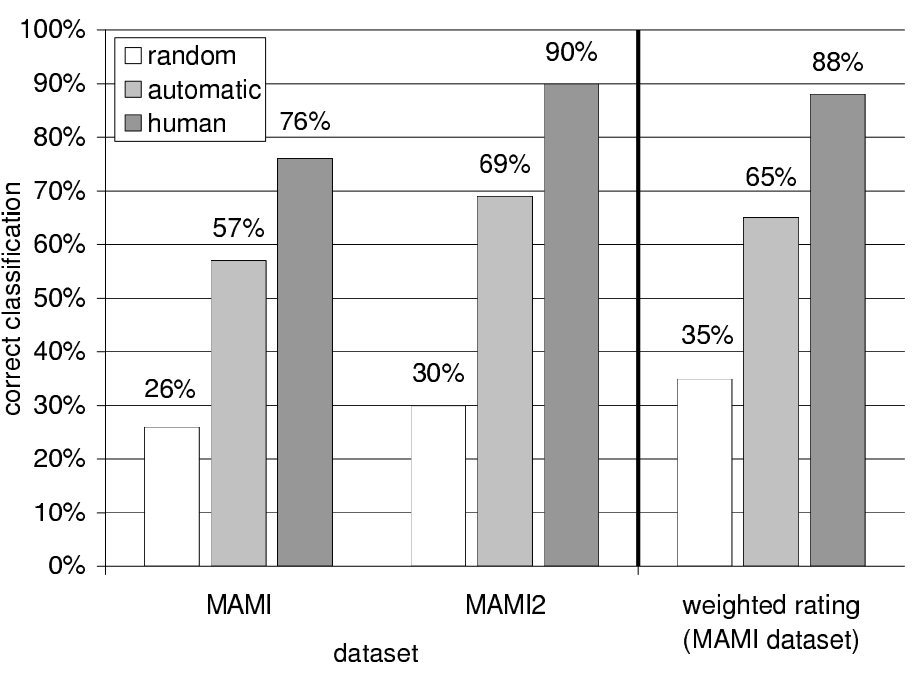
\includegraphics[scale=.2]{graph/genre_human_classification}
                            }
                        \only<2>{
                            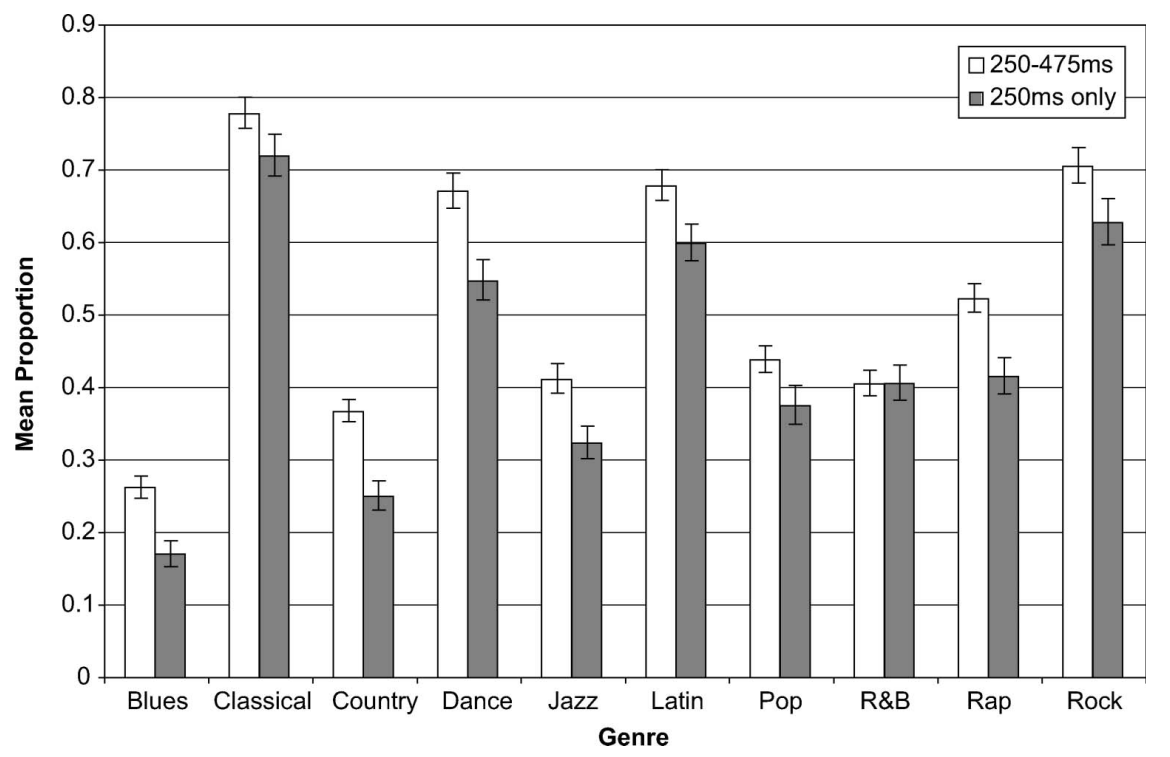
\includegraphics[scale=.15]{graph/genre_shorttime_classification}
                            }
                    \end{figure}
            \end{columns}
            \begin{flushright}plots from \footfullcite{lippens_comparison_2004},\footfullcite{gjerdingen_scanning_2008}\end{flushright}
        \end{frame}
    
    \section[MGC]{automatic musical genre classification}

        \begin{frame}{musical genre classification}{overview}
            \begin{figure}
                \begin{footnotesize}
				\begin{picture}(96,26)
					\setcounter{iXOffset}{0}
					\setcounter{iYOffset}{5}
					\setcounter{iXBlockSize}{28}
					\setcounter{iYBlockSize}{16}
					\setcounter{iYBlockSizeDiv2}{8}
					\setcounter{iDistance}{8}
	
					\addtocounter{iYOffset}{\value{iYBlockSizeDiv2}}
					\addtocounter{iYOffset}{-2}
	
					%\addtocounter{iXOffset}{-1}
					\put(\value{iXOffset}, \value{iYOffset})
						{\text{{\shortstack[c]{Audio\\ Signal}}}}
					\addtocounter{iXOffset}{1}
	
					\addtocounter{iYOffset}{2}
					\addtocounter{iXOffset}{\value{iDistance}}
	
					\put(\value{iXOffset}, \value{iYOffset})
						{\vector(1,0){\value{iDistance}}}
	
					\addtocounter{iXOffset}{\value{iDistance}}
					\addtocounter{iYOffset}{-\value{iYBlockSizeDiv2}}
					
					\put(\value{iXOffset}, \value{iYOffset})
						{\framebox(\value{iXBlockSize}, \value{iYBlockSize}) {{\shortstack[c]{Feature\\ Extraction}}}}
	
					\addtocounter{iXOffset}{\value{iXBlockSize}}
					\addtocounter{iYOffset}{\value{iYBlockSizeDiv2}}
	
					\put(\value{iXOffset}, \value{iYOffset})
						{\vector(1,0){\value{iDistance}}}
	
					\addtocounter{iXOffset}{\value{iDistance}}
					\addtocounter{iYOffset}{-\value{iYBlockSizeDiv2}}
	
					\put(\value{iXOffset}, \value{iYOffset})
						{\framebox(\value{iXBlockSize}, \value{iYBlockSize}) {{\shortstack[c]{Classification}}}}
	
					\addtocounter{iXOffset}{\value{iXBlockSize}}
					\addtocounter{iYOffset}{\value{iYBlockSizeDiv2}}
	
					\put(\value{iXOffset}, \value{iYOffset})
						{\vector(1,0){\value{iDistance}}}
	
					\addtocounter{iXOffset}{\value{iDistance}}
					\addtocounter{iYOffset}{-2}
	
					\addtocounter{iXOffset}{1}
					\put(\value{iXOffset}, \value{iYOffset})
						{\text{{\shortstack[c]{Genre\\ Label}}}}
					
				\end{picture}
\end{footnotesize}
            \end{figure}
            \begin{enumerate}
                    \item	\textbf{feature extraction}
                            \begin{itemize}
                                \item 	compressed, meaningful representation
                            \end{itemize}
                    \bigskip
                    \item<2->	\textbf{classification}
                            \begin{itemize}
                                \item	map or convert feature to comprehensible domain
                            \end{itemize}
            \end{enumerate}
        \end{frame}

    \section{features}
        \begin{frame}{musical genre classification}{feature categories}
            \vspace{-3mm}
            \begin{itemize}
                \item	\textbf{high level similarities}?
                    \begin{itemize}
                        \item	melody, hook lines, bass lines, harmony progression
                        \item	rhythm \& tempo
                        \item	structure
                        \item	instrumentation \& timbre
                    \end{itemize}
                \smallskip
                \item<2->	\textbf{technical feature categories}
                    \begin{itemize}
                        \item	tonal
                        \item	technical
                        \item	timbral
                        \item	temporal
                        \item	intensity
                    \end{itemize}
                \smallskip
                \item<3->       \textbf{extracted features should be}
                    \begin{itemize}
                        \item   extractable (not: time envelope in polyphonic signals)
                        \item   relevant (not: pitch chroma for instrument ID)
                        \item   non-redundant
                        \item   have discriminative power
                    \end{itemize}
            \end{itemize}
        \end{frame}

        \begin{frame}{musical genre classification}{instantaneous features}
            \begin{itemize}
                \item	spectral features (\textbf{timbre}):
                
                    Spectral Centroid, MFCCs, Spectral Flux, \ldots
                \smallskip
                \item<2->	pitch features (\textbf{tonal}):
                
                    pitch chroma distribution/change, \ldots
                \smallskip
                \item<3->	rhythm features (\textbf{temporal}):
                
                    onset density, beat histogram features, \ldots
                \smallskip
                \item<4->	statistical features (\textbf{technical}):
                
                    standard deviation, skewness, zero crossings, \ldots
                \smallskip
                \item<5->	\textbf{intensity} features:
                
                    level variation, number of ``pauses'', \ldots
            \end{itemize}	
        \end{frame}

        \begin{frame}{musical genre classification}{feature extraction process}
            \begin{enumerate}
                \item	extract \textbf{instantaneous features}
                        \only<1>{
                            \vspace{-5mm}
                            \begin{flushright}
                                \includegraphics[scale=.5]{FeatureExtraction}
                            \end{flushright}
                            \vspace{-7mm}
                        }
                \smallskip
                \item<2->	compute \textbf{derived features} (derivatives etc.)
                \smallskip
                \item<3->	compute \textbf{long term features} \& subfeatures per texture window or file
                \smallskip	
                \item<4->	\textbf{normalize} subfeatures
                \smallskip
                \item<5->   (select or) \textbf{transform} subfeatures
                \smallskip
                \item<7->	feature vector $\rightarrow$ \textbf{classifier input}
                            \only<7->{
                            \vspace{-13mm}
                            \begin{flushright}
                                \includegraphics[scale=.5]{FeatureScatter}
                            \end{flushright}
                            }
            \end{enumerate}
            \vspace{20mm}
        \end{frame}
        \begin{frame}{musical genre classification}{long term features 1/2}
            derived from beat histogram\footfullcite{tzanetakis_musical_2002}
            \begin{columns}
            \column{.4\linewidth}
                \begin{itemize}
                    \item   statistical histogram features
                    \item   number and values of top maxima
                    \item   location (relation) of top maxima
                    \item   \ldots
                \end{itemize}
            \column{.6\linewidth}
            \begin{figure}
                \centering
                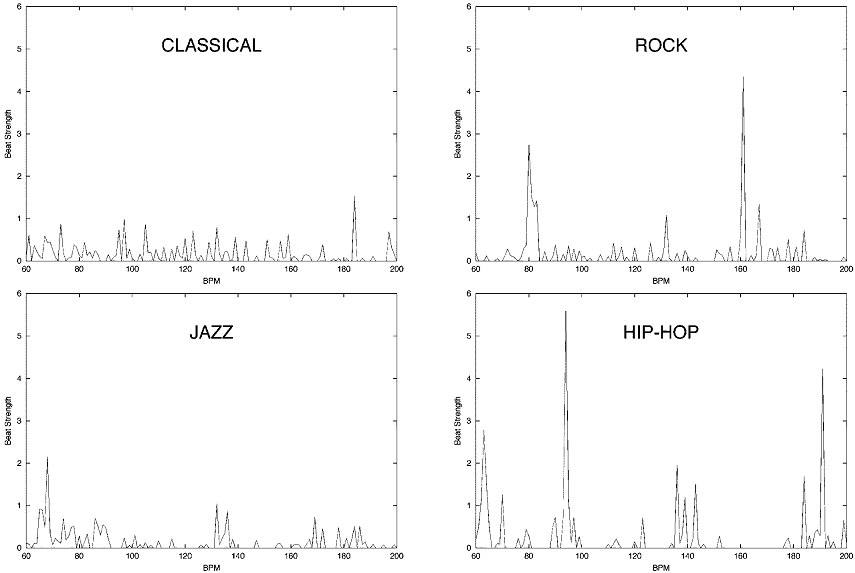
\includegraphics[width=.8\columnwidth]{graph/genre_beat_histogram}
            \end{figure}
            \end{columns}
        \end{frame}
        \begin{frame}{musical genre classification}{long term features 2/2}
            derived from pitch histogram or pitch chroma\footfullcite{tzanetakis_pitch_2002}
            \begin{columns}
            \column{.4\linewidth}
                \begin{itemize}
                    \item   statistical histogram features
                    \item   number and values of top maxima
                    \item   location (relation) of top maxima
                    \item   \ldots
                \end{itemize}
            \column{.6\linewidth}
            \vspace{-3mm}
            \begin{figure}
                \centering
                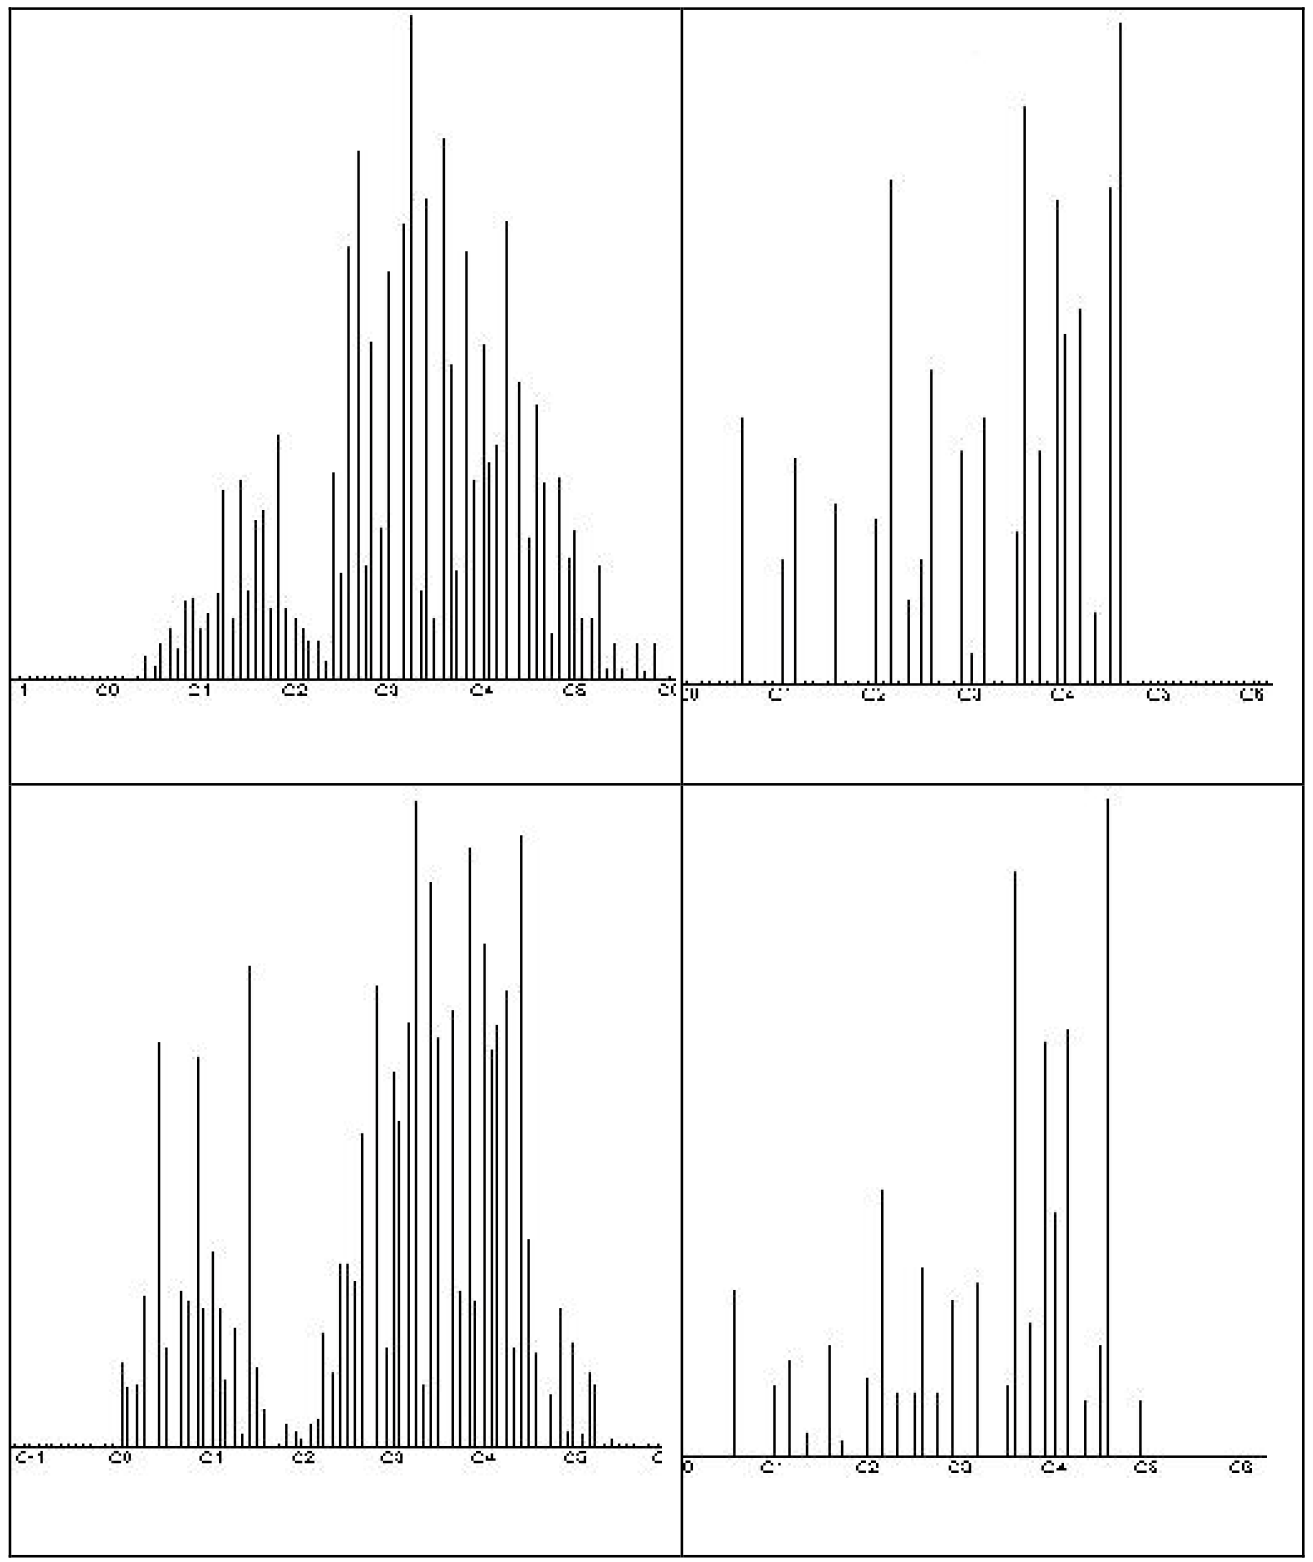
\includegraphics[scale=.12]{graph/genre_pitchhisto}
            \end{figure}
            \end{columns}
        \end{frame}
        \begin{frame}{musical genre classification}{additional possible features}
            \begin{itemize}
                \item	\textbf{stereo features}
                    \begin{itemize}
                        \item	mid channel energy vs.\ side channel energy
                        \item	spectral channel differences
                    \end{itemize}
                \bigskip
                \item<2->	features at \textbf{higher semantic levels}:
                    \begin{itemize}
                        \item   tempo, structure, harmonic complexity, instrumentation
                    \end{itemize}
            \end{itemize}
        \end{frame}

        \begin{frame}{musical genre classification}{results}
            \begin{itemize}
                \item	classification results depend on training set, test set, and number of classes
                \smallskip
                \item<2->	typical range: $\approx 10$ classes $\Rightarrow$ 50--80\%
                \bigskip
                \item<3-> main challenges
                    \begin{itemize}
                        \item   ill-defined genre boundaries
                        \item   non-uniformly distributed classes
                        \item   overfitting through songs from same album or artist
                        \item   \ldots
                    \end{itemize}
            \end{itemize}
        \end{frame}
    \section[example]{real world example}
        \begin{frame}{musical genre classification}{speech/music classification baseline example}
            binary classification task
            \begin{enumerate}
                \item	extract features
                \smallskip
                \item   represent each file with its 2-dimensional feature vector
                \smallskip
                \item   kNN to classify unknown audio files
                \smallskip
                \item   evaluate classification performance
            \end{enumerate}
        \end{frame}

        \begin{frame}{musical genre classification}{speech/music classification example: features 1/2}
            for each audio file
            \begin{enumerate}
                \item<1->	split input signal into (overlapping) blocks
                \only<1>{
                    \vspace{-7mm}
                    \begin{flushright}
                        \begin{footnotesize}
				\begin{picture}(60,40)
					\setcounter{iXOffset}{0}
					\setcounter{iYOffset}{24}
					\setcounter{iXBlockSize}{16}
					\setcounter{iYBlockSize}{4}
					\setcounter{iYBlockSizeDiv2}{2}
					\setcounter{iDistance}{8}

					% block indices
					\put(\value{iXOffset}, \value{iYOffset})
						{\text{{\shortstack[c]{$n$}}}}
					\addtocounter{iYOffset}{-\value{iYBlockSize}}
					\addtocounter{iYOffset}{-\value{iYBlockSizeDiv2}}
					\put(\value{iXOffset}, \value{iYOffset})
						{\text{{\shortstack[c]{$n+1$}}}}
					\addtocounter{iYOffset}{-\value{iYBlockSize}}
					\addtocounter{iYOffset}{-\value{iYBlockSizeDiv2}}
					\put(\value{iXOffset}, \value{iYOffset})
						{\text{{\shortstack[c]{$n+2$}}}}
					\addtocounter{iYOffset}{-\value{iYBlockSize}}
					\addtocounter{iYOffset}{-\value{iYBlockSizeDiv2}}
					\put(\value{iXOffset}, \value{iYOffset})
						{\text{{\shortstack[c]{$n+3$}}}}

					% audio time line
					\setcounter{iYOffset}{30}
					\setcounter{iXOffset}{5}
					\put(\value{iXOffset}, \value{iYOffset})
						{\vector(1,0){50}}
	
					% blocks
					\addtocounter{iXOffset}{5}
					\addtocounter{iYOffset}{-\value{iYBlockSize}}
					\addtocounter{iYOffset}{-\value{iYBlockSizeDiv2}}
					\put(\value{iXOffset}, \value{iYOffset})
						{\framebox(\value{iXBlockSize}, \value{iYBlockSize})}
					\addtocounter{iXOffset}{5}
					\addtocounter{iYOffset}{-\value{iYBlockSize}}
					\addtocounter{iYOffset}{-\value{iYBlockSizeDiv2}}
					\put(\value{iXOffset}, \value{iYOffset})
						{\framebox(\value{iXBlockSize}, \value{iYBlockSize})}
					\addtocounter{iXOffset}{5}
					\addtocounter{iYOffset}{-\value{iYBlockSize}}
					\addtocounter{iYOffset}{-\value{iYBlockSizeDiv2}}
					\put(\value{iXOffset}, \value{iYOffset})
						{\framebox(\value{iXBlockSize}, \value{iYBlockSize})}
					\addtocounter{iXOffset}{5}
					\addtocounter{iYOffset}{-\value{iYBlockSize}}
					\addtocounter{iYOffset}{-\value{iYBlockSizeDiv2}}
					\put(\value{iXOffset}, \value{iYOffset})
						{\framebox(\value{iXBlockSize}, \value{iYBlockSize})}

	
					% lengths
					\linethickness{.03mm}
					\setcounter{iYOffset}{34}
					\setcounter{iXOffset}{10}
					\put(\value{iXOffset}, \value{iYOffset})
						{\line(0,-1){12}}
					\put(\value{iXOffset}, \value{iYOffset})
						{\vector(1,0){1}}
					\addtocounter{iXOffset}{5}
					\put(\value{iXOffset}, \value{iYOffset})
						{\line(0,-1){18}}
					\put(\value{iXOffset}, \value{iYOffset})
						{\vector(-1,0){1}}
					\addtocounter{iXOffset}{5}
					\addtocounter{iXOffset}{5}
					\put(\value{iXOffset}, \value{iYOffset})
						{\line(0,-1){30}}
					\put(\value{iXOffset}, \value{iYOffset})
						{\vector(1,0){1}}
					\addtocounter{iXOffset}{\value{iXBlockSize}}
					\put(\value{iXOffset}, \value{iYOffset})
						{\line(0,-1){30}}
					\put(\value{iXOffset}, \value{iYOffset})
						{\vector(-1,0){1}}

					\put(11, 34)
						{\text{$\mathcal{H}$}}
					\put(32, 34)
						{\text{$\mathcal{K}$}}
					\put(56, 28)
						{\text{$i$}}
				\end{picture}
\end{footnotesize}
	
                    \end{flushright}			
                }
                \item<2->	compute 2 feature series (spectral centroid, RMS)
                \only<2>{
                    \vspace{-1mm}
                    \begin{flushright}
                        \includegraphics[scale=.5]{FeatureSpectralCentroid}	
                    \end{flushright}			
                }
                \item<3->	aggregate feature series to one value per file
                    \begin{itemize}
                        \item	\textit{mean} of Spectral Centroid $\mu_\mathrm{SC}$
                        \only<3>{
                            \begin{equation*}
                                \mu_\mathrm{SC} = \frac{1}{N}\sum_{\forall n}{v_\mathrm{SC}(n)}
                            \end{equation*}
                            }
                        \item	\textit{standard deviation} of RMS $\sigma_\mathrm{RMS}$
                        \only<3>{
                            \begin{equation*}
                                \sigma_\mathrm{RMS} = \sqrt{\frac{1}{N}\sum_{\forall n}{(v_\mathrm{RMS}(n)-\mu_\mathrm{RMS})^2}}
                            \end{equation*}
                            }
                    \end{itemize}
                \item<4->	represent each file as 2-dimensional vector
                        \only<4>{
                        \begin{equation*}
                            \big(\mu_\mathrm{SC}, \sigma_\mathrm{RMS}\big)^\mathrm{T}
                        \end{equation*}
                    }
            \end{enumerate}				
        \end{frame}

        \begin{frame}{musical genre classification}{speech/music classification example: features 2/2}
            \figwithmatlab{Featurespace}
        \end{frame}

        \begin{frame}{musical genre classification}{speech/music classification example: training set}
            \begin{itemize}
                \item	use \textbf{dataset} annotated as speech and music:
                    \begin{itemize}
                        \item	requirements
                            \begin{itemize}
                                \item	large compared to number of features
                                \item	representative for use case (diverse)
                            \end{itemize}
                        \item	here (toy example):
                            \begin{itemize}
                                \item	64 speech files
                                \item	64 music files
                            \end{itemize}
                    \end{itemize}
                \bigskip
                \item	extract the features for the dataset
                    \begin{itemize}
                        \item   centroid mean
                        \item   rms std
                    \end{itemize}
                \bigskip
                \item	use 3NN classifier
                \bigskip
                \item	procedure: Leave-One-Out-Cross-Validation
            \end{itemize}
        \end{frame}


        \begin{frame}{musical genre classification}{speech/music classification example: results (kNN)}
            \begin{itemize}
                \item   \textbf{confusion matrix}:
                    \begin{table}
                        \centering
                        \begin{tabular}{l|cc|ccccccccc} %{\textwidth}{@{\extracolsep{\fill}}ccccccccccccc}
                            \bf{\emph{}}	 & \bf{\emph{speech}}	 & \bf{\emph{music}} & \# files	 \\ 
                             \hline
                            \bf{gt speech}	 & $\mathbf{51}$	 & $13$	 & $64$\\
                            \bf{gt music}	 & $11$	 & $\mathbf{53}$ & $64$
                        \end{tabular}
                    \end{table}
                \item<2->$\Rightarrow$ \textbf{classification rate}: 
                    \begin{equation*}
                        \frac{53 + 54}{64 + 64} = 81.25\%
                    \end{equation*}
                \smallskip
                \item<3->   single feature classification results
                    \begin{itemize}
                        \item	Spectral Centroid: $63.28\%$
                        \item	RMS: $73.44\%$
                    \end{itemize}
            \end{itemize}
            \addreference{matlab source: \href{https://github.com/alexanderlerch/ACA-Code/blob/master/ExampleMusicSpeechClassification.m}{matlab/ExampleMusicSpeechClassification.m}}
                        
        \end{frame}
    
    \section{summary}
        \begin{frame}{summary}{lecture content}
            \begin{itemize}
                \item   \textbf{musical genre}
                    \begin{itemize}
                        \item   ill-defined, subjective, no general agreement
                        \item   some human agreement
                    \end{itemize}
                \bigskip
                \item   \textbf{MGC: features}
                    \begin{itemize}
                        \item   from all possible categories as all categories might depend on genre
                        \item   timbre seems most meaningful feature
                    \end{itemize}
                \bigskip
                \item   \textbf{MGC: classifier}
                    \begin{itemize}
                        \item   any classifier works, and most have been used
                    \end{itemize}
                \bigskip
                \item   \textbf{MGC: standard baseline}
                    \begin{enumerate}
                        \item   MFCCs
                        \item   SVM
                    \end{enumerate}
            \end{itemize}
            \inserticon{summary}
        \end{frame}
\end{document}
